% Un hablante para test, lo demás para train
%\subsection{Un hablante para test y los demás para train}
\subsection{Clasificación por muestra}
\label{un_hablante_para_test_los_demas_train}

\usetikzlibrary{shapes.geometric}

\tikzset{myshade/.style={minimum size=.4cm,shading=radial,inner color=white,outer color={#1!90!gray}}}
\newcommand\mycirc[1][]{\tikz\node[circle,myshade=#1]{};}

Vamos a definir un modelo de test distinto. Este va a enfatizar más la idea del hablante y de cómo distinguirlo. Para cada fold generado, excluiremos un hablante y entrenaremos con todos los demás. Luego testeamos contra ese hablante excluido. Este nuevo esquema evita que tengamos grabaciones repetidas en los grupos de tests. Podemos ver este esquema en la tabla \ref{HPTDT_esq_cv}. Este esquema también es conocido como \textbf{validación cruzada dejando uno fuera} (en inglés: Leave-one-out cross-validation)

En nuestro conjunto de datos tenemos 27 hablantes: 19 de Buenos Aires y 8 de Córdoba. Vamos a tener 27 folds distintos para cada uno de ellos. Cada uno de estos folds va a excluir todos los audios de este hablante, por eso cuando nos referimos a un hablante nos referimos a todos los audios grabados por él.

\begin{center}
	\mycirc[blue] Hablante para train \mycirc[red] Hablante para test
\end{center}

\begin{table}[H]
	\centering
	\begin{tabular}{cccccccccccc}
		& \multicolumn{11}{c}{\textit{Número de hablante}} \\
		& 1 & 2 & 3 & 4 & 5 & 6 & 7 & ... & 25 & 26 & 27 \\
		\hline \\
		Fold 1 &\mycirc[red] & \mycirc[blue] & \mycirc[blue]  & \mycirc[blue]  & \mycirc[blue]  & \mycirc[blue]  & \mycirc[blue] & ... & \mycirc[blue] & \mycirc[blue] & \mycirc[blue]  \\
		
		Fold 2 &\mycirc[blue] & \mycirc[red] & \mycirc[blue]  & \mycirc[blue]  & \mycirc[blue]  & \mycirc[blue]  & \mycirc[blue] & ... & \mycirc[blue] & \mycirc[blue] & \mycirc[blue]  \\
		
		Fold 3 &\mycirc[blue] & \mycirc[blue] & \mycirc[red]  & \mycirc[blue]  & \mycirc[blue]  & \mycirc[blue]  & \mycirc[blue] & ... & \mycirc[blue] & \mycirc[blue] & \mycirc[blue]  \\
	
		\multicolumn{11}{c}{\textit{...}}	\\
		
		Fold 27 &\mycirc[blue] & \mycirc[blue] & \mycirc[blue]  & \mycirc[blue]  & \mycirc[blue]  & \mycirc[blue]  & \mycirc[blue] & ... & \mycirc[blue] & \mycirc[blue] & \mycirc[red]   \\
	
	\end{tabular}
	\caption{Esquema de validación cruzada}
	\label{HPTDT_esq_cv}
\end{table}
		
\subsubsection{Resultados}

En la tabla \ref{HPTDT_clas_xval_porHab} podemos observar los resultados de clasificación. Expresamos solamente el promedio de clasificación correcta de los folds para cada clasificador. No resulta relevante mostrar el porcentaje de clasificación correcta para cada fold. 

\begin{table}[H]
	\centering
	\begin{tabular}{|l|c|c|c|c|c|c|}
		\hline
		\textbf{}  & \textbf{Zero Rule} & \textbf{Ripper} & \textbf{C4.5} & \textbf{SVM} & \textbf{NaiveBayes} \\ \hline
		%\textbf{Fold 1}  &  &  &  &  &  \\ \hline
		%\hline \hline
		\textbf{Promedio} & 70.37  & 69.47 & 70.37 & 71.34 & 71.46 \\ \hline
	\end{tabular}
	\caption{Clasificación correcta en porcentaje}
	\label{HPTDT_clas_xval_porHab}
\end{table}

Llama la atención que todos los clasificadores tuvieron porcentajes muy cercanos. Esto lo analizaremos más adelante. 

Realizamos los test estadísticos de Wilcoxon y Test t de Student para este modelo de test. En este caso, las muestras de test son independientes entre sí. Estos resultados se pueden observar en la tabla  \ref{HPTDT_res_tests_wilcoxon_student}.

\begin{table}[H]
	\centering
	\begin{tabular}{|l|c|c|c|c|c|c|}
		\hline
		\textbf{}  & \textbf{Student Test} & \textbf{Wilcoxon Test} \\ \hline
		\textbf{ZeroR y Ripper}  & 0.5816 & 0.6234 \\ \hline
		\textbf{ZeroR y C4.5}  & 1 & 1 \\ \hline
		\textbf{ZeroR y NaiveBayes}  & 0.4383 & 0.4042 \\ \hline
		\textbf{ZeroR y SVM}  & 0.4302 & 0.2646 \\ \hline
	\end{tabular}
	\caption{Resultados de cada test representado en p-valor}
	\label{HPTDT_res_tests_wilcoxon_student}
\end{table}

Los valores expresados corresponden al p-valor. Todos los clasificadores pasaron el test Shapiro-Wilk, entonces podemos afirmar que los resultados de cada clasificador corresponden a una distribución Normal. A pesar de esto, realizamos ambos tests estadísticos para cada uno. Estos test mostraron que las diferencias entre cada clasificador y el baseline no son estadísticamente significativos.

\subsubsection{Análisis de los clasificadores construidos}

Analizamos los clasificadores armados para cada fold. En este modelo de test también los clasificadores Support vector machine y NaiveBayes utilizaron todos los atributos ponderando cada uno por valores escalares. El clasificador C4.5 tuvo también una performance pobre por tener un árbol de un nivel solo. 

Veamos el clasificador Ripper para el fold 4. Este es el conjunto de reglas que generó:

\begin{flushleft}
	\begin{itemize}
		\item $(FON\_rr\_norm <= -6.901) and (ACU\_AverageRR\_7 <= 11.23) => place=cba (18.0/3.0)$ \\
		\item $(FON\_ll\_norm <= -7.975) and (ACU\_AverageLL\_6 <= 4.308) => place=cba (15.0/0.0)$
		\item $else => place=bsas (222.0/49.0)$
	\end{itemize}
\end{flushleft}

Notamos que sigue utilizando los atributos temporales y en menor medida los atributos acústicos.

% hablar de los problemas encontrados y cómo mejorarlos con el próximo cross-validation 

\subsubsection{Características del modelo de test}

Si bien este modelo de test simplificó mucho la forma de modelar, nos sigue mostrando resultados llamativos. 

El clasificador Zero Rule sigue teniendo muy buen rendimiento solamente por tener un conjunto de datos desequilibrado. También el clasificador C4.5 posee muy bajo performance y su árbol de clasificación sigue siendo muy pobre.  

%Ver bien el mail de Miguel
Analizando el algoritmo del clasificador C4.5 notamos que el árbol generado puede ser muy pobre si en sus datos de entrenamiento hay muchos valores desconocidos. 

Recordemos que el algoritmo C4.5 para armar el árbol de clasificación va tomando el atributo con mayor ganancia de información y agregándolo como un nuevo nodo al árbol. Luego descarta el atributo ya elegido y se llama recursivamente en cada rama. 

Si hay muchas instancias con atributos desconocidos, pocos atributos tendrán buena ganancia de información y no podrá armar un árbol extenso. Recordemos que, para un hablante, cada uno de sus audios sólo define atributos para la frase grabada. Si en la grabación no se extrae ese atributo, quedará con valor desconocido. 

\begin{table}[H]
	\centering
	\begin{tabular}{|l|l|ccccccccc|}
		\hline
		\multicolumn{2}{|l|}{Atributos} & A1 & A2 & A3 & A4 & A5 & A6 & A7 & ... & AN \\
		\hline 
		\textbf{Hablante 1} & \textbf{Audio1} & 1 & 2 & ? & ? & ? & ? & ? & ... & 2 \\
		& \textbf{Audio2} & ? & ? & 1 & 3 & 4 & ? & ? & ... & ? \\
		& \textbf{Audio3} & ? & ? & ? & ? & ? & 4 & 2 &  ... & ? \\
		\hline
	\end{tabular}
	\caption{Ejemplo de atributos para un hablante}
	\label{HPTDT_hablante_ej}
\end{table}

Veamos un ejemplo: en la tabla \ref{HPTDT_hablante_ej} podemos ver los atributos extraídos de un hablante ficticio. Supongamos que este hablante grabó sólo 3 audios. En el primer audio se define los atributos A1, A2 y AN. En el segundo audio se define A3, A4 y A5. En último audio se define los atributos A6 y A7. Todos los demás atributos poseen valores desconocidos, pero en realidad corresponden a un mismo hablante. Si bien, para ese audio en particular es un atributo desconocido, la realidad es que corresponde a un mismo hablante y podemos inferirlo de otro audio grabado por él. Deberíamos tener alguna forma de evitar tener valores desconocidos cuando pueden ser extraídos de otro audio.

Suponemos que el mal rendimiento de C4.5 viene de la mano de los valores desconocidos. Creemos que si tenemos menor cantidad de valores desconocidos esta performance mejorará. Pensamos esta idea luego de leer cómo funciona los árboles de decisión del libro \cite{DataMining-PracticalMachineLearningTools} \footnote{En la página 194 está la explicación que nos ayudó a razonar esta idea.}. En la sección \ref{prom_los_atributos_de_cada_hablante} probaremos otro modelo de test que intente evitar tener tantos valores desconocidos. 


% % % % % % % % % % % % % % % % % % % % % % % % % % % % % % % % % %
% Correcciones a agregar
Correcciones a agregar


\begin{center}
	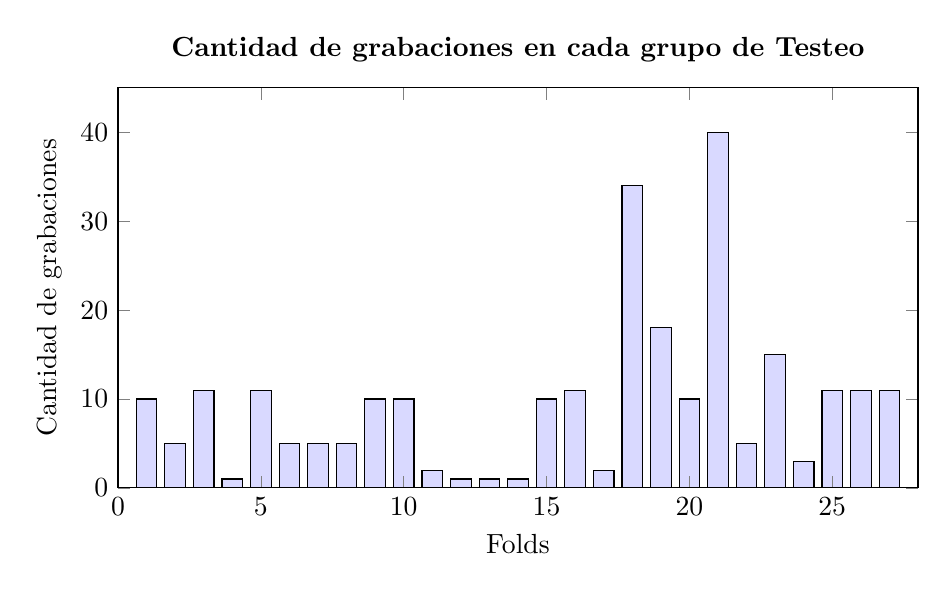
\begin{tikzpicture}
	
	\begin{axis}[
	title={\textbf{Cantidad de grabaciones en cada grupo de Testeo}},
	xlabel={Folds},
	ylabel={Cantidad de grabaciones},
	scale only axis,
	width=4in,
	height=2in,
	xmin=0, xmax=28,
	ymin=0, ymax=45,
	axis on top]
	\addplot[
	ybar,
	fill=blue!15,
	bar width=0.102874in, 
	bar shift=0in,
	draw=black] 
	plot coordinates{ 
		(1, 10)(2, 5)(3, 11)(4, 1)(5, 11)(6, 5)(7, 5)(8, 5)(9, 10)(10,10)(11,2)(12,1)(13,1)(14,1)(15,10)(16,11)(17,2)(18,34)(19,18)(20,10)(21,40)(22,5)(23,15)(24,3)(25,11)(26,11)(27,11) 
	};
	
	\end{axis}
	\end{tikzpicture}	
\end{center}


\textbf{Promedio de porcentaje correcto en cada fold:}
\[
{ \sum_{i=1}^{\text{\# de folds}} \text{Porcentaje instancias correctas en fold \textit{i}}
	\over
	\text{\# de folds}
}
\]

{\small 	\begin{table}[H]
		\centering
		\begin{tabular}{|l|c|c|c|c|c|c|}
			\hline
			\textbf{}  & \textbf{Zero Rule} & \textbf{Ripper} & \textbf{C4.5} & \textbf{SVM} & \textbf{NaiveBayes} \\ \hline
			%\textbf{Fold 1}  &  &  &  &  &  \\ \hline
			%\hline \hline
			\textbf{Promedio} & 70  & 69 & 70 & 71 & 71 \\ \hline
		\end{tabular}
		\caption{Clasificación correcta en porcentaje}
		\label{HPTDT_clas_xval_porHab}
	\end{table}}
	
	\textbf{Promedio de instancias correctas sobre instancias totales:}
	\small
	\[
	{ \sum_{i=1}^{\text{\# de folds}} \text{Cantidad de instancias correctas en fold \textit{i}}
		\over
		\text{\# de instancias}
	}
	\]
	
	{\small 	\begin{table}[H]
			\centering
			\begin{tabular}{|l|c|c|c|c|c|c|}
				\hline
				\textbf{}  & \textbf{Zero Rule} & \textbf{Ripper} & \textbf{C4.5} & \textbf{SVM} & \textbf{NaiveBayes} \\ \hline
				%\textbf{Fold 1}  &  &  &  &  &  \\ \hline
				%\hline \hline
				\textbf{Promedio} & 69  & 63 & 69 & 70 & 65 \\ \hline
			\end{tabular}
			\caption{Clasificación correcta en cantidad de instancias}
			\label{HPTDT_clas_xval_porHab}
		\end{table}}
		
		
		Árbol de decisión generado por C4.5 para cualquier fold para clasificación por muestra.
		
		\dirtree{%
			.1 root.
			.2 $bsas (249.0/68.0)$.
		}
		